\chapter{Project Design}

This chapter presents the requirements of the system, its architecture, how the avatar model was selected, adapted to Bangla and improved, and the project plan.

\section{Requirement Analysis}
The system has two very different computational profiles. \textit{Training} the avatar model is done once per avatar and needs a datacentre-class GPU; we used Google Colab (NVIDIA A100 and L4). \textit{Running} the system must fit on consumer hardware: the avatar renderer runs locally on a laptop NVIDIA RTX 3050 with 4~GB of memory, while conversational reasoning is handled by a cloud API. The project also requires Bangla audiovisual data for training and evaluation, and enough local storage for video frames, landmarks and audio features.


\subsection{Functional and Nonfunctional Requirements}

\subsubsection{Functional Requirements}

\begin{enumerate}
    \item \textbf{Interface:} The system captures the user's microphone audio in a web browser and displays the avatar's video and audio reply, with a live transcript.

    \item \textbf{Secured Real-Time Communication Layer (RTC):} Audio and video are streamed between the user and the system over LiveKit, with access tokens issued by a token server.

    \item \textbf{Conversational Processing Module:} The agent detects the end of the user's turn, understands the Bangla request, and generates a spoken Bangla reply that keeps the conversation history.

    \item \textbf{Speech Output:} The reply is produced directly as Bangla speech by the speech-to-speech conversational model.

    \item \textbf{Talking-Head Video Generation \& Streaming:} The avatar server turns the reply audio into lip-synchronised video frames, streams them in step with the audio, and plays an idle animation when the avatar is not speaking.
\end{enumerate}


\subsubsection{Non-Functional Requirements}

\begin{enumerate}
    \item \textbf{Availability:} The system is accessible whenever the server is running, with minimal downtime.

    \item \textbf{Security:} Users are authenticated through session tokens.

    \item \textbf{Performance \& Quality:} The system answers within 1--2 seconds of the user finishing speaking, and the avatar renders at no less than 25 frames per second.

    \item \textbf{Reliability:} The system runs on a consumer laptop GPU without exhausting its memory.

    \item \textbf{Linguistic Robustness:} Bangla speech is transcribed in Bangla script and answered in natural, formal-register Bangla.

    \item \textbf{Modularity \& Scalability:} The conversational agent, the real-time media layer and the avatar renderer are decoupled, so each can be upgraded or replaced independently.
\end{enumerate}


\subsection{System Diagram}
The system diagram is depicted in Figure~\ref{fig:SystemDiagram}, which gives a high-level overview of our system.
\begin{figure}[H]
    \centering
    \begin{tikzpicture}[
        node distance=0.9cm and 1.2cm,
        box/.style={draw=axisgrey, fill=restsoft, rounded corners, align=center, minimum width=4.6cm, minimum height=1.05cm, font=\small, text=inkc},
        local/.style={box},
        cloud/.style={box, dashed},
        alapon/.style={box, draw=alaponblue, fill=alaponsoft, line width=0.9pt, text=alapondark},
        arr/.style={{Stealth[length=2mm]}-{Stealth[length=2mm]}, thick, draw=inkc},
        barr/.style={arr, draw=alaponblue},
        lbl/.style={font=\footnotesize, fill=white, inner sep=1.5pt, text=inkgrey}]
      \node[box, fill=white] (user) {User};
      \node[local, below=of user] (browser) {Browser client\\ microphone, avatar video, transcript};
      \node[local, right=of browser, minimum width=3.4cm] (token) {Token server\\ (Flask)};
      \node[cloud, below=of browser] (lk) {LiveKit Cloud\\ real-time audio and video};
      \node[local, below=of lk] (agent) {Bangla agent\\ LiveKit Agents, Silero VAD};
      \node[cloud, right=of agent, minimum width=3.4cm] (gemini) {Gemini 3.1 Flash Live\\ (cloud API)};
      \node[alapon, below=of agent] (avatar) {Avatar server\\ \textbf{Alapon} on the laptop GPU};
      \draw[arr] (user) -- node[lbl, right] {speech / avatar} (browser);
      \draw[arr] (browser) -- node[lbl, above] {token} (token);
      \draw[arr] (browser) -- node[lbl, right] {audio / video} (lk);
      \draw[arr] (lk) -- node[lbl, right] {audio / video} (agent);
      \draw[arr] (agent) -- node[lbl, above] {speech} (gemini);
      \draw[barr] (agent) -- node[lbl, right, text=alapondark] {reply audio / frames} (avatar);
    \end{tikzpicture}

    \vspace{0.3em}
    {\footnotesize\color{inkgrey} Dashed border: cloud service. Blue: Alapon, the avatar model, running on the laptop.}
    \caption{System Diagram}
    \label{fig:SystemDiagram}
\end{figure}

\subsection{Sequence Diagram}
The sequence diagram is depicted in Figure~\ref{fig:SequenceDiagram}, which shows the order of interactions between the components during one conversational turn.
\begin{figure}[H]
    \centering
    \resizebox{\textwidth}{!}{%
    \begin{tikzpicture}[
        head/.style={draw=axisgrey, rounded corners, fill=restsoft, align=center, minimum width=2.1cm, minimum height=0.9cm, font=\small, text=inkc},
        ahead/.style={head, draw=alaponblue, fill=alaponsoft, text=alapondark, line width=0.9pt},
        msg/.style={-{Stealth[length=2mm]}, thick, draw=inkc},
        ret/.style={msg, dashed},
        bmsg/.style={msg, draw=alaponblue},
        bret/.style={bmsg, dashed},
        lbl/.style={font=\footnotesize, above, inner sep=1.5pt, align=center, text=inkgrey},
        note/.style={draw=axisgrey, fill=restsoft, font=\footnotesize, align=center, inner sep=2pt, text=inkc},
        anote/.style={note, draw=alaponblue, fill=alaponsoft, text=alapondark}]
      \foreach \x/\name/\txt in {0/U/User, 2.6/B/Browser\\client, 5.2/T/Token\\server, 7.8/L/LiveKit, 10.4/A/Bangla\\agent, 13.0/G/Gemini\\Live}{
        \node[head] (\name) at (\x,0) {\txt};
        \draw[restgrey, thick] (\x,-0.45) -- (\x,-12.6);
      }
      \node[ahead] (V) at (15.6,0) {Avatar server\\ (Alapon)};
      \draw[alaponblue!45, thick] (15.6,-0.45) -- (15.6,-12.6);
      \draw[msg] (2.6,-1.1) -- node[lbl] {request token} (5.2,-1.1);
      \draw[ret] (5.2,-1.8) -- node[lbl] {token} (2.6,-1.8);
      \draw[msg] (2.6,-2.5) -- node[lbl] {join room} (7.8,-2.5);
      \draw[msg] (0,-3.2) -- node[lbl] {speaks Bangla} (2.6,-3.2);
      \draw[msg] (2.6,-3.9) -- node[lbl] {microphone audio} (7.8,-3.9);
      \draw[msg] (7.8,-4.6) -- node[lbl] {user audio} (10.4,-4.6);
      \node[note] at (10.4,-5.4) {VAD: end of turn\\ after 0.55 s of silence};
      \draw[msg] (10.4,-6.3) -- node[lbl] {user speech} (13.0,-6.3);
      \draw[ret] (13.0,-7.0) -- node[lbl] {reply speech + transcript} (10.4,-7.0);
      \draw[bmsg] (10.4,-7.7) -- node[lbl, text=alapondark] {reply audio (24 kHz PCM)} (15.6,-7.7);
      \node[anote] at (15.6,-8.5) {Alapon renders\\ lip-synced frames};
      \draw[bret] (15.6,-9.4) -- node[lbl, text=alapondark] {frames + audio segments} (10.4,-9.4);
      \draw[msg] (10.4,-10.1) -- node[lbl] {publish audio + video} (7.8,-10.1);
      \draw[msg] (7.8,-10.8) -- node[lbl] {audio + video} (2.6,-10.8);
      \draw[msg] (2.6,-11.5) -- node[lbl] {avatar speaks} (0,-11.5);
      \node[note, minimum width=13.6cm] at (8.9,-12.2) {Idle animation is streamed whenever the avatar is not speaking};
    \end{tikzpicture}}
    \caption{Sequence Diagram of the Proposed System}
    \label{fig:SequenceDiagram}
\end{figure}




\subsection{UI Design}

\begin{figure}[H]
    \centering
    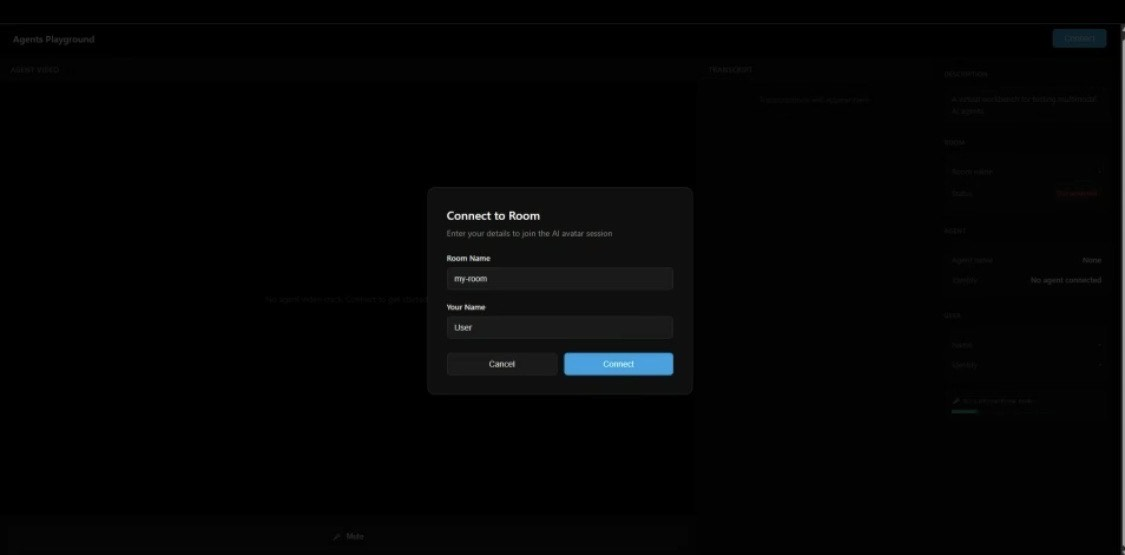
\includegraphics[width=0.8\textwidth]{UI1.jpeg}
    \caption{User Interface of our System}
    \label{fig: User Interface of our System}
\end{figure}


\begin{figure}[H]
    \centering
    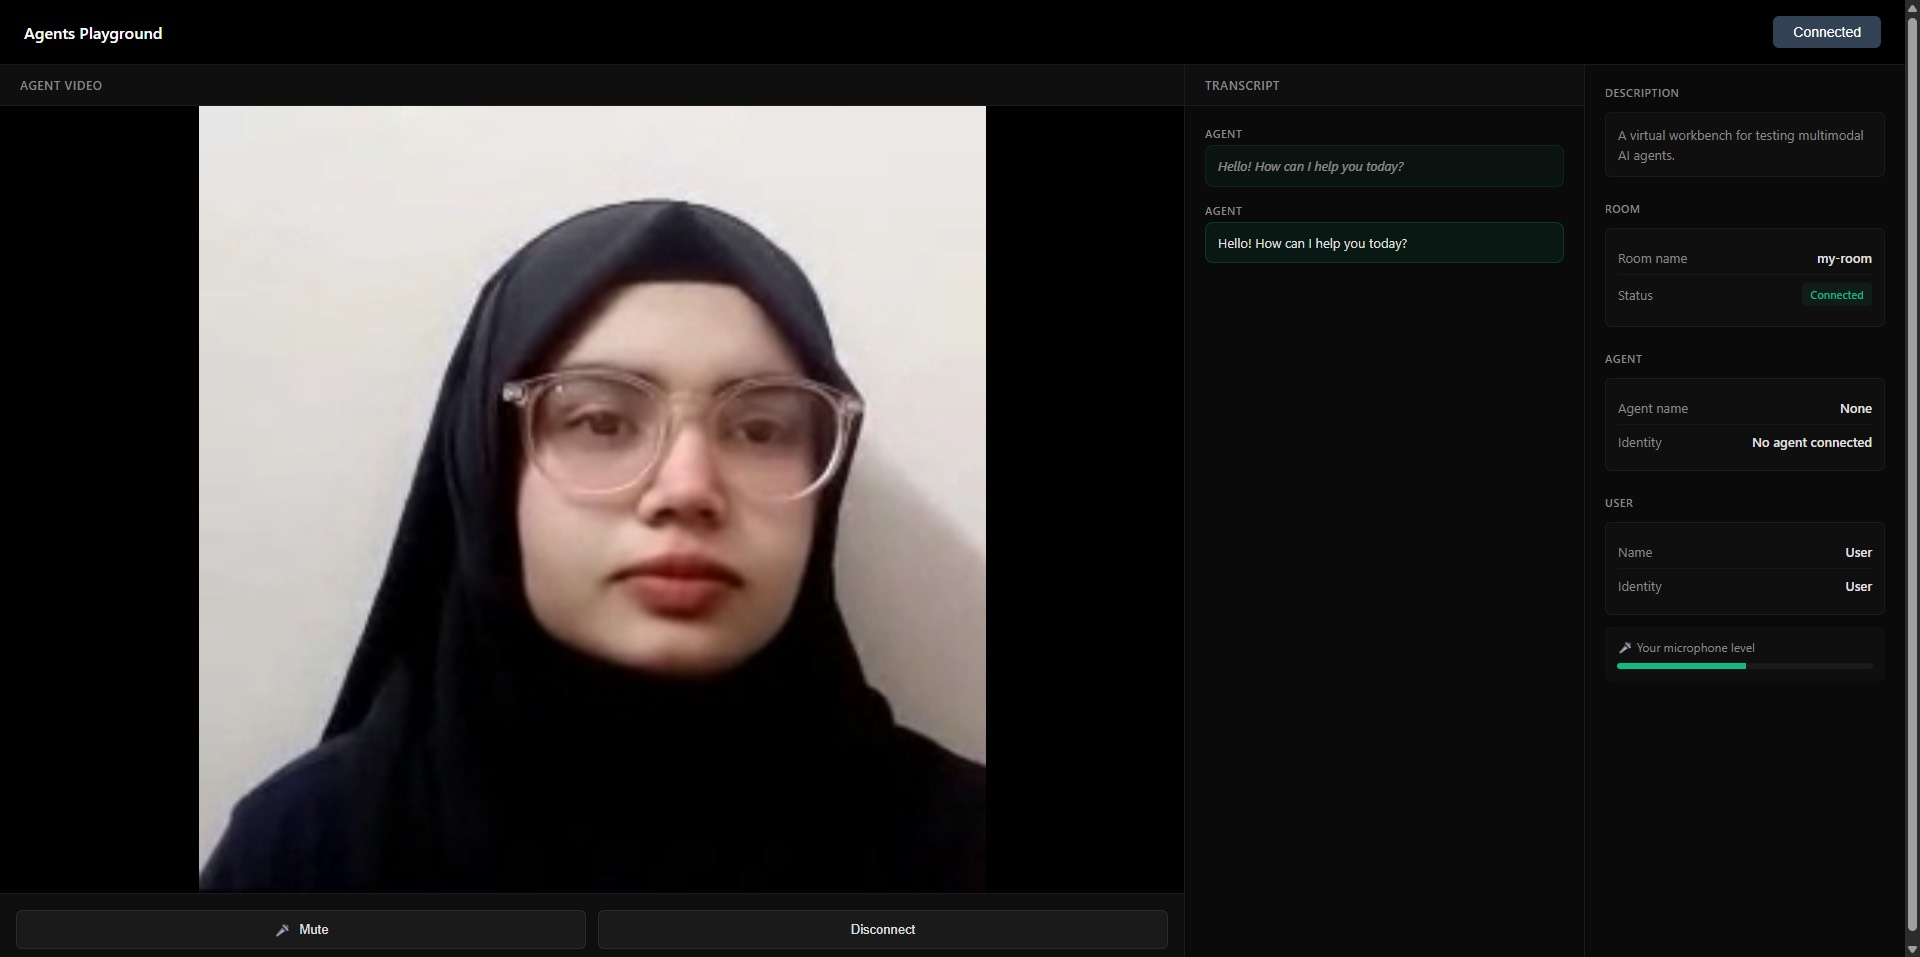
\includegraphics[width=0.8\textwidth]{UI2.jpeg}
    \caption{User Interface of our System}
    \label{fig: User Interface of our System 2}
\end{figure}


\section{Detailed Methodology and Design}

This section describes the architecture of the delivered system, how the design evolved, the Bangla conversational agent, the avatar rendering server, and how the avatar model was selected, adapted to Bangla and improved.

\subsubsection{Overall System Architecture}

The system is a voice-to-voice-and-video pipeline:

\begin{center}
\textit{Speech $\rightarrow$ Conversational model $\rightarrow$ Speech $\rightarrow$ Audio features $\rightarrow$ Lip-synchronised video}
\end{center}

\noindent
The user speaks Bangla in the browser. The audio reaches the agent over LiveKit. The agent's conversational model produces a spoken Bangla reply, which is sent to the avatar server. The avatar server converts the reply audio into lip-synchronised video frames and streams them back, and the agent publishes the audio and video together to the user through LiveKit. The components are independent processes connected by LiveKit and WebSockets, so each can be developed, debugged and replaced separately.


\begin{figure}[H]
    \centering
    \resizebox{\textwidth}{!}{%
    \begin{tikzpicture}[
        comp/.style={draw=axisgrey, rounded corners, fill=white, align=center, font=\small, minimum height=0.95cm, minimum width=3.3cm, text=inkc},
        acomp/.style={comp, draw=alaponblue, fill=alaponsoft, text=alapondark, line width=0.9pt},
        layer/.style={draw=axisgrey, dashed, rounded corners, inner sep=8pt, fill=restsoft},
        ttl/.style={font=\small\bfseries, anchor=south west, inner sep=2pt, text=inkc},
        arr/.style={-{Stealth[length=2mm]}, thick, draw=inkc},
        barr/.style={arr, draw=alaponblue},
        lbl/.style={font=\footnotesize, fill=white, inner sep=1.5pt, align=center, text=inkgrey}]
      % client layer
      \node[comp] (browser) at (0,0) {Browser client\\ mic, video, transcript};
      \node[comp] (token) at (4.2,0) {Token server\\ (Flask)};
      % rtc
      \node[comp, dashed, minimum width=7.5cm] (lk) at (2.1,-2.1) {LiveKit Cloud (WebRTC): real-time audio and video};
      % agent
      \node[comp] (vad) at (0,-4.4) {Silero VAD\\ end of turn: 0.55 s};
      \node[comp] (sess) at (4.2,-4.4) {Gemini session\\ bn-BD, persona, phrases};
      \node[comp, dashed] (gem) at (9.4,-4.4) {Gemini 3.1 Flash Live\\ speech-to-speech (cloud)};
      % avatar
      \node[comp] (feat) at (0,-7.0) {Streaming audio\\ features};
      \node[acomp] (unet) at (4.2,-7.0) {\textbf{Alapon}\\ U-Net renderer};
      \node[comp] (jpeg) at (8.4,-7.0) {JPEG frames +\\ segment protocol};
      \node[comp] (idle) at (8.4,-8.6) {Idle frame cache};
      \begin{scope}[on background layer]
        \node[layer, fit=(browser)(token)] (L1) {};
        \node[layer, fit=(lk)] (L2) {};
        \node[layer, fit=(vad)(sess)] (L3) {};
        \node[layer, fill=alaponsoft!45, draw=alaponblue!60, fit=(feat)(unet)(jpeg)(idle)] (L4) {};
      \end{scope}
      \node[ttl] at (L1.north west) {Client layer};
      \node[ttl] at (L2.north west) {Real-time communication layer};
      \node[ttl] at (L3.north west) {Bangla agent (LiveKit Agents)};
      \node[ttl, text=alapondark] at (L4.north west) {Avatar server (FastAPI, laptop GPU)};
      \draw[arr] (token) -- (browser);
      \draw[arr, {Stealth[length=2mm]}-{Stealth[length=2mm]}] (browser) -- (browser |- lk.north);
      \draw[arr, {Stealth[length=2mm]}-{Stealth[length=2mm]}] (vad |- lk.south) -- (vad);
      \draw[arr] (vad) -- node[lbl, above] {turn} (sess);
      \draw[arr, {Stealth[length=2mm]}-{Stealth[length=2mm]}] (sess) -- node[lbl, above] {speech} (gem);
      \draw[barr] (sess) -- node[lbl, right, text=alapondark] {reply audio\\ 24 kHz PCM} (sess |- L4.north);
      \draw[barr] (feat) -- (unet);
      \draw[barr] (unet) -- (jpeg);
      \draw[barr] (jpeg.north) -- ++(0,1.2) -| node[lbl, pos=0.25, text=alapondark] {frames + audio} (sess.south east);
      \draw[arr] (idle) -- (jpeg);
    \end{tikzpicture}}
    \caption{System Architecture}
    \label{fig:SystemArchitecture}
\end{figure}

\noindent
\textbf{How the design evolved.} The FYDP-1 design was a cascade of three separate services: Whisper speech recognition through a Gradio API, Gemini 2.5 Flash for text reasoning, and Microsoft Edge TTS (\texttt{bn-IN-TanishaaNeural}) for speech synthesis. Each stage added its own latency, so we moved to Gemini's speech-to-speech ``native audio'' model, which removed the separate recognition and synthesis stages. That model, however, slowed down as a conversation went on: its reply time grew from 8 seconds to 66 seconds within five turns. Switching to \texttt{gemini-3.1-flash-live-preview} kept the reply time constant, and this is the model used in the final system.

\vspace{0.5em}

\subsubsection{Real-Time Communication Layer and Agent Control}

The agent is built on the LiveKit Agents framework \cite{livekitagents}. It creates the LiveKit session, greets the user, and then listens continuously, routing the user's audio to the conversational model and the reply to the avatar server. It manages the session lifecycle and user interruptions, so the interaction behaves like a conversation rather than a request--response exchange. A small Flask server issues the LiveKit access tokens used by the browser.

\vspace{0.5em}

\subsubsection{Bangla Conversational Agent}

The conversational model \cite{geminilive} receives the user's speech directly and replies in speech. Three Bangla-specific problems appeared that do not occur in English, and each needed its own fix.

\begin{itemize}
    \item \textbf{Wrong script in the transcript.} By default the model detected the language afresh on every utterance. With short turns of 0.6--1.8 seconds, phonetic overlap between Bangla, Hindi and Punjabi, and English loanwords, the same speaker's words came back in Devanagari, Gurmukhi and Roman script within a single session. We pinned the input language to \texttt{bn-BD}.
    \item \textbf{Turns cut off mid-question.} Bangla speakers pause mid-sentence, and the default end-of-turn detection answered half a question. We run a local voice-activity detector (Silero \cite{silero2021}) with the end-of-turn silence set to 0.55 seconds, long enough to survive a natural Bangla pause.
    \item \textbf{Technical vocabulary pulled towards English.} Terms such as ``\bn{মেশিন লার্নিং}'' and ``ChatGPT'' repeatedly shifted recognition away from Bangla. We supply them as biasing phrases.
\end{itemize}

\noindent
The agent's persona, ``Redwan'', answers only in Bangla, in the formal register (\bn{আপনি}), and keeps established technical terms in their usual form.

\vspace{0.5em}

\subsubsection{Avatar Rendering Server}

The avatar server is a FastAPI application with WebSocket endpoints for audio in and video out. At 25 frames per second it has a budget of 40~ms per frame.

\begin{itemize}
    \item \textbf{Streaming audio features.} The model was trained on audio features extracted from whole recordings, but live audio arrives in chunks. Extracting features chunk by chunk shifts the timeline slightly at every boundary and slowly desynchronises the lips. Our streaming feature extractor produces the same features as offline extraction: it resamples with a fixed phase, recomputes mel frames from a hop-aligned tail with eight frames of context, and emits a feature only once all of its audio has arrived.
    \item \textbf{Segment protocol.} Each reply segment carries its frame count and its audio, so the client knows exactly how many frames to expect and plays them against the audio.
    \item \textbf{Audio never waits for video.} If a frame is late the previous frame is repeated, because a gap in the voice is far more noticeable than a repeated frame.
    \item \textbf{Cached source frames and idle animation.} Decoded video frames and their landmarks are cached in memory, and idle frames are pre-rendered, so the GPU is free to render speech when it arrives.
\end{itemize}

\vspace{0.5em}

\subsubsection{Selecting the Avatar Model}
\label{sec:selection}

The avatar model must render at least 25 frames per second on a 4~GB laptop GPU while the rest of the system is running, and its lips must follow Bangla speech. We chose SyncTalk\_2D for its size and speed, and confirmed the choice by running the published lip-sync systems that have public code and weights on the same 31-second Bangla clip (Table~\ref{tab:candidates}). Their lip-sync results are in Section~\ref{sec:comparison}.

\begin{table}[H]
\centering
\caption{Candidate avatar models against the project requirements}
\label{tab:candidates}
\renewcommand{\arraystretch}{1.3}
\begin{tabular}{|p{3.1cm}|p{4.4cm}|r|p{3.2cm}|}
\hline
\textbf{Model} & \textbf{Type} & \textbf{Checkpoint file} & \textbf{Time for the 31 s clip (T4)$^{*}$} \\
\hline
\textbf{SyncTalk\_2D} \cite{synctalk2d} & 2D, person-specific & \textbf{49 MB} & \textbf{2 min 33 s} \\
\hline
Wav2Lip \cite{prajwal2020wav2lip} & 2D, person-generic & 436 MB$^{\dagger}$ & 9 min 06 s \\
\hline
IP-LAP \cite{zhong2023iplap} & 2D, person-generic & 475 MB & not timed \\
\hline
MuseTalk 1.5 \cite{zhang2024musetalk} & 2D latent, person-generic & 3,400 MB & about 15 min \\
\hline
LatentSync 1.5 \cite{li2024latentsync} & 2D latent diffusion, person-generic & 5,072 MB & about 30 min \\
\hline
InsTaG \cite{li2025instaglearningpersonalized3d} & 3D Gaussian Splatting, person-specific & -- & not run \\
\hline
\end{tabular}

\vspace{0.3em}
{\footnotesize $^{*}$Offline generation on a cloud T4 GPU, including each system's one-off preprocessing and video file reading and writing; this is not a measure of live speed. $^{\dagger}$Wav2Lip's file also stores training optimiser state, so its model weights are smaller than the file. IP-LAP: its two checkpoints together.}
\end{table}

\begin{figure}[H]
    \centering
    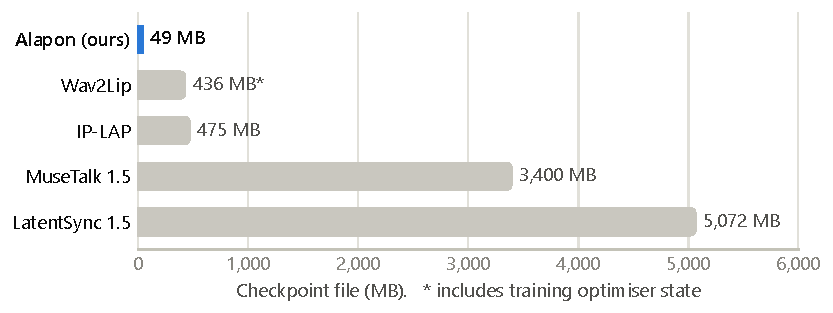
\includegraphics[width=\textwidth]{fig_model_size.pdf}
    \caption{Checkpoint size of the candidate models}
    \label{fig:modelsize}
\end{figure}

\noindent
SyncTalk\_2D has the smallest model and generated the clip fastest. LatentSync's model file alone is larger than the laptop's 4~GB of GPU memory, and MuseTalk's nearly fills it. InsTaG was ruled out because 3D Gaussian Splatting training and rendering exceed the 4~GB laptop budget. The person-generic systems can animate any face without training; SyncTalk\_2D's cost is that it must be trained for each face (about five minutes of video and seven hours of training), which is acceptable for an avatar that represents one fixed speaker. Being person-specific also means the speaker's identity, eyes and head motion come directly from real video; only the mouth is generated.

\vspace{0.5em}

\subsubsection{Alapon: Adapting SyncTalk\_2D to Bangla}

SyncTalk\_2D \cite{synctalk2d} is a 2D U-Net that receives two images, a reference frame of the speaker and the current frame with the mouth region blacked out, together with audio features, and paints the mouth back in (Figure~\ref{fig:Alapon}). \textbf{Alapon} is SyncTalk\_2D adapted to Bangla and improved in the following ways.

\begin{figure}[H]
    \centering
    \resizebox{0.95\textwidth}{!}{%
    \begin{tikzpicture}[
        blk/.style={draw=axisgrey, fill=restsoft, rounded corners, align=center, font=\small, minimum height=1cm, minimum width=3.2cm, text=inkc},
        arr/.style={-{Stealth[length=2mm]}, thick, draw=inkc},
        lbl/.style={font=\footnotesize, fill=white, inner sep=1.5pt, align=center, text=inkgrey}]
      % inputs
      \node[blk] (ref) at (0,2.2) {Reference frame\\ (one fixed frame)};
      \node[blk] (msk) at (0,0.6) {Current frame,\\ mouth and jaw hidden};
      \node[blk] (aud) at (0,-1.0) {Audio features\\ (streamed live)};
      \node[blk, draw=alaponblue, fill=alaponsoft, text=alapondark, line width=0.9pt, minimum height=3.8cm] (unet) at (4.6,0.6) {\textbf{Alapon}\\ U-Net};
      \node[blk, fill=white] (out) at (8.8,0.6) {Generated mouth\\ pasted into frame};
      \node[blk, dashed, fill=white] (sync) at (4.6,-2.4) {Bangla lip-sync expert\\ (training only)};
      \draw[arr] (ref) -- (unet.west |- ref);
      \draw[arr] (msk) -- (unet);
      \draw[arr, draw=alaponblue] (aud) -- (unet.west |- aud);
      \draw[arr, draw=alaponblue] (unet) -- (out);
      \draw[arr, dashed, draw=axisgrey] (out.south) |- node[lbl, pos=0.75] {sync loss} (sync.east);
      % mask inset: orange = the jaw the original mask left visible
      \begin{scope}[shift={(11.6,-0.9)}]
        \node[font=\footnotesize\bfseries, text=leakorange] at (0.7,3.5) {Original mask};
        \draw[axisgrey, fill=white] (0,0) rectangle (1.4,3.2);
        \fill[inkc] (0.15,0.25) rectangle (1.25,1.7);
        \fill[leaksoft] (0.15,0) rectangle (1.25,0.25);
        \draw[leakorange, thick] (0.15,0) rectangle (1.25,0.25);
        \node[font=\scriptsize, text=leakorange, align=center] at (0.7,-0.28) {jaw visible};
        \node[font=\footnotesize\bfseries, text=alapondark] at (2.6,3.5) {Alapon};
        \draw[axisgrey, fill=white] (1.9,0) rectangle (3.3,3.2);
        \fill[inkc] (2.05,0) rectangle (3.15,1.7);
        \node[font=\scriptsize, text=white] at (2.6,0.9) {hidden};
        \node[font=\scriptsize, text=alapondark, align=center] at (2.6,-0.28) {jaw hidden};
      \end{scope}
    \end{tikzpicture}}
    \caption{Alapon: inputs, output and the change to the mouth mask}
    \label{fig:Alapon}
\end{figure}

\noindent
\textbf{1. Bangla training data.} The avatar is trained on 7,717 frames (about 5.1 minutes) of a Bangla speaker, \texttt{redwan}, at 25~fps and 1080$\times$1080. The recording is split into contiguous intervals: frames 0--6170 for training, 6171--6941 for validation, and 6942--7713 (772 frames) for testing. Contiguous intervals are used because neighbouring frames are almost identical, and a random split would put near-copies of test frames into training.\\

\noindent
\textbf{2. Bangla lip-sync expert.} During training, a SyncNet ``expert'' judges whether the generated mouth matches the audio. We retrained the expert on the Bangla speaker with contrastive sampling: half of all training pairs are mismatched, so the expert must learn to tell a correct mouth from a shifted one. The avatar was trained against this Bangla expert, with the sync loss switched on from epoch 5 at a weight of 0.03.\\

\noindent
\textbf{3. Streaming audio features} for the live system, described above.\\

\noindent
\textbf{4. Multilingual audio encoder (XLS-R).} The default audio features come from an audio--visual encoder trained on English. We also tried XLS-R \cite{babu2022xlsr}, a speech encoder pre-trained on 128 languages including Bangla, in place of these features. It did not work (Section~\ref{sec:xlsr}), so Alapon uses the default features.\\

\noindent
\textbf{5. Closing the model's performance gaps.} While training the Bangla model we found that its mouth moved even when the audio was silent, and its lips did not close fully on \bn{প}, \bn{ব}, \bn{ম}. Investigating this revealed four gaps in the SyncTalk\_2D model that held back its performance (Table~\ref{tab:gaps}). Alapon addresses all four. Only the first is measured directly on its own (Section~\ref{sec:maskfix}); the other three are design and training issues that we corrected together.

\begin{table}[H]
\centering
\caption{Gaps in the SyncTalk\_2D model and how Alapon addresses them}
\label{tab:gaps}
\renewcommand{\arraystretch}{1.3}
\begin{tabular}{|p{4.2cm}|p{5.3cm}|p{3.7cm}|}
\hline
\textbf{Gap in the model} & \textbf{Effect on performance} & \textbf{How Alapon addresses it} \\
\hline
\textbf{The mouth mask does not cover the jaw.} The mouth region should be fully hidden, but the bottom ten rows of the face crop (the chin and jaw) stay visible in training and in use. & The model reads mouth opening from the visible jaw instead of the audio, so the mouth moves during silence and lip closures are weak. With audio and reference held constant, this ten-pixel strip produced \textbf{91\% of all mouth motion}. & Mask extended to cover the jaw (Section~\ref{sec:maskfix}). \\
\hline
\textbf{The lip-sync expert learns only from matching audio--video pairs.} & It never sees an out-of-sync example, so it approves every mouth and gives no useful training signal, consistent with the FYDP-1 observation that SyncNet scores stayed near 1.0 at every offset. & Expert retrained with mismatched pairs (item 2). \\
\hline
\textbf{The lip-sync loss is weighted 10$\times$.} & Together with the gap above, a strong training signal that carries no real information about synchronisation. & Weight 0.03, switched on from epoch 5. \\
\hline
\textbf{Training and use see different reference frames.} & A mismatch between what the model learns and what it sees at run time. & One fixed reference frame in both. A control run showed this changes leakage by only 1\%. \\
\hline
\end{tabular}
\end{table}

\noindent
\textbf{6. A clean training split.} While preparing the final training runs we also found that training had drawn frames, including reference frames, from the whole video, test interval included. Training now uses only the training interval, and the interval is recorded with each trained model. The models evaluated in this report were trained before this change; Section~\ref{sec:testing} explains which results this affects.\\

\noindent
\textbf{7. Bangla phoneme-to-viseme mapping.} A \textit{viseme} is a visually distinct mouth shape; several phonemes can share one. Table~\ref{tab:viseme} maps the Bangla sound inventory to eleven visemes.

\begin{table}[H]
\centering
\caption{Bangla phoneme-to-viseme mapping}
\label{tab:viseme}
\renewcommand{\arraystretch}{1.3}
\begin{tabular}{|p{1.1cm}|p{4.2cm}|p{4.3cm}|p{3.6cm}|}
\hline
\textbf{Viseme} & \textbf{Mouth shape} & \textbf{Bangla letters} & \textbf{Phonemes (IPA)} \\
\hline
V0 & Rest, lips closed & (silence, pause) & -- \\
\hline
V1 & Lips pressed together & \bn{প ফ ব ভ ম} & {\ipafont /p pʰ b bʱ m/} \\
\hline
V2 & Lips apart, neutral; tongue at teeth or ridge & \bn{ত থ দ ধ ট ঠ ড ঢ ড় ঢ় ন ণ ল র স ৎ} & {\ipafont /t̪ t̪ʰ d̪ d̪ʱ ʈ ʈʰ ɖ ɖʱ ɽ ɽʱ n l r s/} \\
\hline
V3 & Lips slightly protruded & \bn{চ ছ জ ঝ য শ ষ} & {\ipafont /tʃ tʃʰ dʒ dʒʱ ʃ/} \\
\hline
V4 & Neutral; jaw follows the vowel & \bn{ক খ গ ঘ ঙ ং হ} & {\ipafont /k kʰ g gʱ ŋ ɦ/} \\
\hline
V5 & Spread, close & \bn{ই ঈ} & {\ipafont /i/} \\
\hline
V6 & Spread, mid-open & \bn{এ}, \bn{অ্যা} & {\ipafont /e æ/} \\
\hline
V7 & Wide open, jaw dropped & \bn{আ} & {\ipafont /a/} \\
\hline
V8 & Open, slightly rounded & \bn{অ} & {\ipafont /ɔ/} \\
\hline
V9 & Rounded, mid & \bn{ও} & {\ipafont /o/} \\
\hline
V10 & Rounded and protruded, close & \bn{উ ঊ} & {\ipafont /u/} \\
\hline
\end{tabular}
\end{table}

\noindent
\todo{have a team member confident in Bangla phonetics check Table~\ref{tab:viseme}}\\

\noindent
The mapping makes three properties of Bangla explicit. Aspiration (\bn{ক}/\bn{খ}, \bn{ত}/\bn{থ}, \bn{দ}/\bn{ধ}) does not change lip shape, so each aspirated consonant shares a viseme with its unaspirated pair. Dental and retroflex consonants (\bn{ত}/\bn{ট}, \bn{দ}/\bn{ড}) differ in tongue position rather than lip shape and also share a viseme. Vowel length in spelling (\bn{ই}/\bn{ঈ}, \bn{উ}/\bn{ঊ}) and nasalisation (\bn{চন্দ্রবিন্দু}) are not visible on the lips, and diphthongs (\bn{ঐ}, \bn{ঔ}) are sequences of two vowel visemes. These distinctions must therefore be carried by the audio, not by the mouth shape. The mapping defines the classes for the sound-level evaluation in Section~\ref{sec:phoneme}; using it as a training signal is future work.

\vspace{0.5em}

\subsubsection{Bangla Audiovisual Corpus}

We also collected a corpus of Bangla speech video: 38 videos, of which 28 from 24 speakers (2.78 hours) passed quality filtering. It was not used to train Alapon, which is person-specific and uses a single speaker; six of its speakers are used as unseen test audio in Section~\ref{sec:phoneme}.

\vspace{0.5em}

\subsubsection{Performance and System Configuration}

The system runs in a hybrid configuration: the avatar renderer, the agent and the browser client run locally, and conversational reasoning is handled by the Gemini API. The runtime machine has an AMD Ryzen 7 5800H processor, 8~GB of RAM, and an NVIDIA RTX 3050 Laptop GPU with 4~GB of memory. Training ran on Google Colab A100 and L4 GPUs; the benchmark of published systems ran on Colab A100, L4 and T4 GPUs. Measured speed and latency are reported in Section~\ref{sec:speed}.


\section{Project Plan}

The project was carried out as a staged development with parallel work, iterative validation and continuous documentation.\\

\noindent
The first phase defined the problem, analysed the requirements and reviewed the literature on Bangla speech processing, real-time voice assistants and audio-driven lip synchronisation. It established the technical basis and feasibility of the system.\\

\begin{figure}[H]
    \centering
    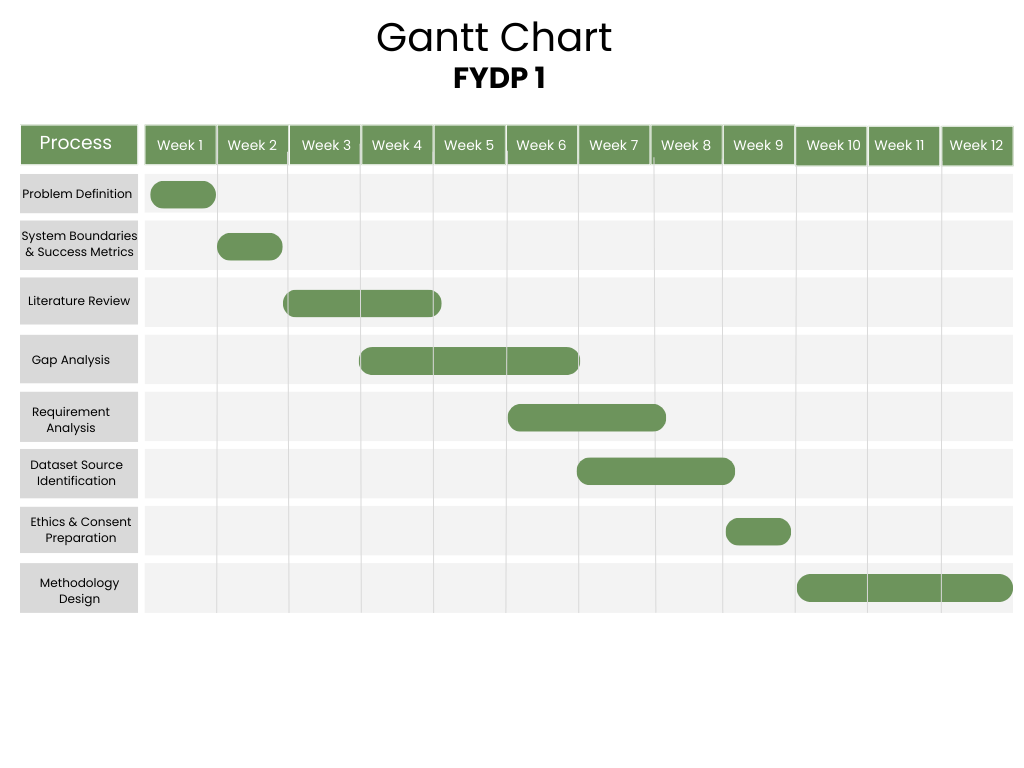
\includegraphics[width=0.8\textwidth]{Gantt Chart for FYDP - 1.png}
    \caption{Gantt Chart for FYDP - 1}
    \label{fig: Gantt Chart for FYDP - 1}
\end{figure}

\noindent
The second phase designed the architecture and built the English baseline: the voice pipeline, real-time streaming over LiveKit, and the integration of the avatar renderer. Modules were built and tested separately before being combined, and continuous testing checked real-time performance, latency and stability.\\

\begin{figure}[H]
    \centering
    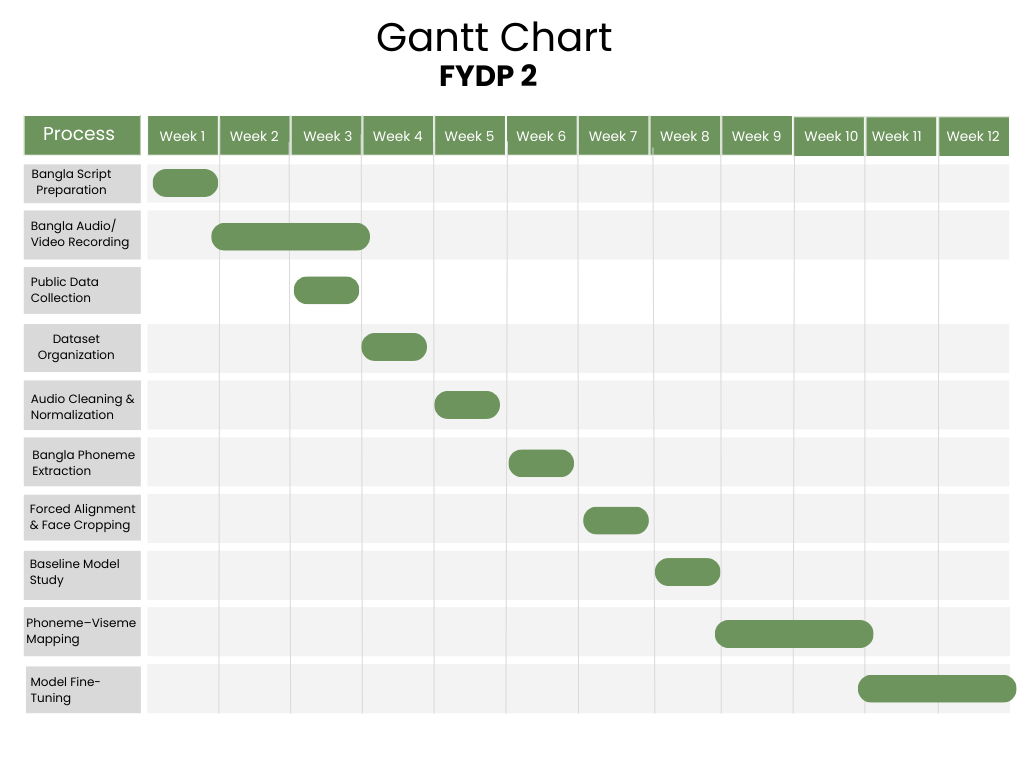
\includegraphics[width=0.8\textwidth]{Gantt Chart for FYDP - 2.png}
    \caption{Gantt Chart for FYDP - 2}
    \label{fig: Gantt Chart for FYDP - 2}
\end{figure}

\noindent
The third phase moved the system to Bangla and built Alapon: the Bangla agent, the choice of avatar model, training on Bangla video, the Bangla lip-sync expert, closing the model's performance gaps, a trial of the XLS-R encoder, the benchmark of published systems on Bangla and HDTF video, and the Bangla sound-level evaluation. The final step was the preparation of this report and the start of the journal paper.\\

\begin{figure}[H]
    \centering
    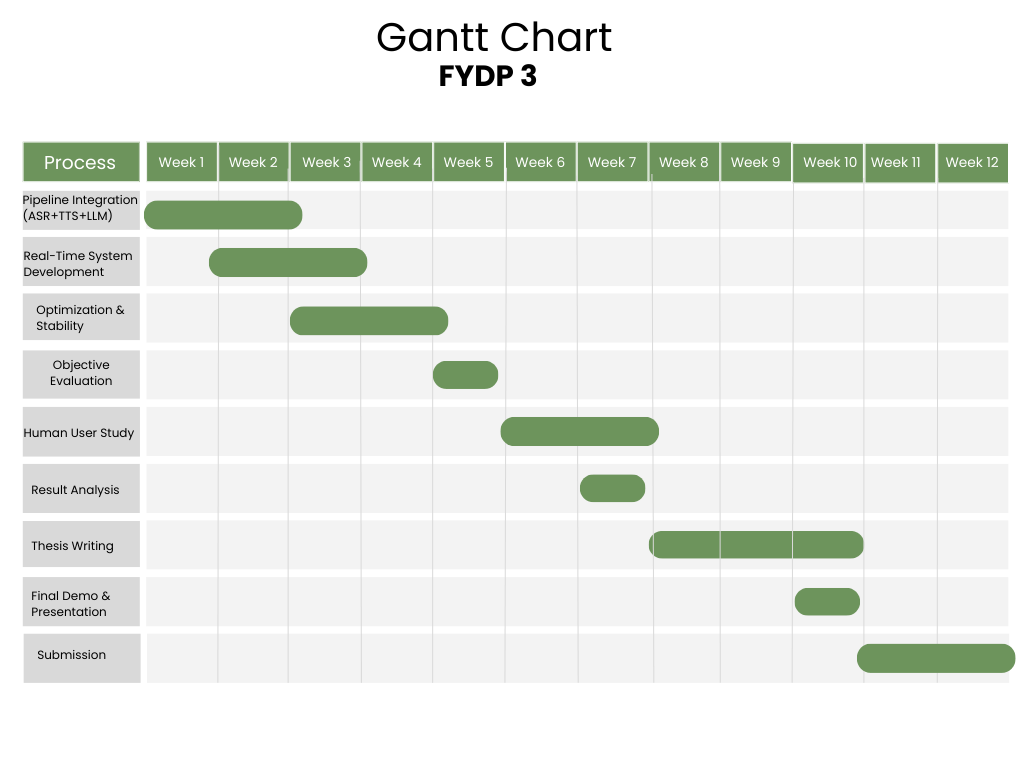
\includegraphics[width=0.8\textwidth]{Gantt Chart for FYDP - 3.png}
    \caption{Gantt Chart for FYDP - 3}
    \label{fig: Gantt Chart for FYDP - 3}
\end{figure}



\section{Task Allocation}

The work was divided among the six team members so that development of the pipeline, research and experiments, and documentation could proceed in parallel. The table below shows the distribution of roles and the main areas each member focused on.\\

\begin{table}[H]
\centering
\caption{Distribution of Project Responsibilities}
\renewcommand{\arraystretch}{1.3}
\begin{tabular}{|p{2.5cm}|p{3.5cm}|p{7.5cm}|}
\hline
\textbf{Team Member} & \textbf{Primary Role} & \textbf{Key Responsibilities \& Deliverables} \\
\hline

\textbf{Member 1} & Systems Architect + R\&D &
Integration of the conversational agent pipeline; LiveKit infrastructure; system-level latency and performance. \\
\hline

\textbf{Member 2} & R\&D and Creative &
Bangla speech and lip-sync research; comparative analysis; project imagery and posters. \\
\hline

\textbf{Member 3} & Documentation \& Lead Coordinator &
Report structure; project coordination; quality control of academic content and consistency. \\
\hline

\textbf{Member 4} & Module Developer &
Implementation of system modules; data preparation for model training; unit testing. \\
\hline

\textbf{Member 5} & Validation Engineer &
Debugging; performance monitoring; iterative refinement of system responses. \\
\hline

\textbf{Member 6} & Implementation Support &
UI/UX components; validation of software deliverables; integration testing. \\
\hline

\end{tabular}
\label{tab:project_responsibilities}
\end{table}




\section{Summary}

This chapter set out the requirements and design of the real-time Bangla conversational avatar. The requirements separate a one-off training workload, which uses cloud GPUs, from a runtime workload that must fit on a consumer laptop. The architecture connects a browser client, a Bangla speech-to-speech agent and an avatar rendering server through LiveKit and WebSockets; it was reached through a cascaded prototype and a native-audio model whose latency grew during long conversations.\\

\noindent
SyncTalk\_2D was chosen as the avatar model because it is the only candidate small and fast enough for a laptop, and the benchmark of published alternatives confirmed the choice. Building Alapon from it involved Bangla training data, a Bangla lip-sync expert, streaming audio features, closing four gaps in the model's design and training, a clean training split, and a Bangla phoneme-to-viseme mapping; a multilingual XLS-R encoder was also tried but did not work. The project plan and task allocation describe how the six-member team divided this work. Chapter~4 reports the implementation and results.\\
